\documentclass[11pt,a4paper]{article}
\newcommand{\gls}[1]{#1\textsubscript{G}}
\usepackage[utf8]{inputenc}
\usepackage[italian]{babel}
\usepackage{geometry}
\usepackage{graphicx}
\usepackage{float}
\usepackage{tabularx}
\usepackage{booktabs}
\usepackage{caption}
\usepackage{hyperref}
\usepackage{fancyhdr}
\usepackage{lastpage}
\usepackage{longtable}

\usepackage{array}
\newcolumntype{M}[1]{>{\centering\arraybackslash}m{#1}}

\geometry{margin=2.5cm}

% Intestazione e piè di pagina
\pagestyle{fancy}
\fancyhf{}
\renewcommand{\headrulewidth}{0pt}
\fancyfoot[C]{\thepage\ di \pageref{LastPage}}

\begin{document}

% Prima pagina - Intestazione
\begin{titlepage}
    \centering
    
    % Logo Università
    \begin{figure}[H]
        \centering
        
\includegraphics[width=0.3\textwidth]{../logoUnipd.jpg}
    \end{figure}
    
    \vspace{0.5cm}
    
    \textbf{\Large Università degli Studi di Padova} \\
    \vspace{0.2cm}
    \textbf{Laurea in Informatica} \\
    \vspace{0.2cm}
    \textbf{Corso di Ingegneria del Software} \\
    \vspace{0.2cm}
    \textbf{Anno Accademico 2025/2026} \\
    
    \vspace{1cm}
    
    % Logo gruppo
    \begin{figure}[H]
        \centering
        
\includegraphics[width=0.2\textwidth]{../LogoByteMe.jpg}
    \end{figure}
    
    \vspace{0.5cm}
    
    \textbf{\Large Gruppo ByteMe} \\
    \vspace{0.2cm}
    \texttt{byteme2025swe@gmail.com} \\
    
    \vspace{1cm}
    
    \textbf{\Huge \gls{Specifica Tecnica}} \\
    
    \vspace{1.5cm}
    
    \begin{table}[H]
        \centering
        \begin{tabular}{|l|p{5cm}|}
            \hline
            \textbf{Versione} & 0.0.8 \\
            \hline
            \textbf{Stato} & In corso \\
            \hline
            \textbf{Redazione} & Giulia Barzon, Joseph Grant, Chiara Grossele, Matteo Cuogo \\
            \hline
            \textbf{\gls{Verifica}} & Verificato \\
            \hline
            \textbf{Approvazione} & Da approvare\\
            \hline
            \textbf{Proprietario} & ByteMe \\
            \hline
            \textbf{Uso} & Esterno \\
            \hline
            \textbf{Destinatari} & Prof. Tullio Vardanega \\ & Prof. Riccardo Cardin \\
            \hline
        \end{tabular}
    \end{table}
    
    \vfill
\end{titlepage}

% Seconda pagina - Versionamento
\thispagestyle{empty}
\section*{Registro dei Cambiamenti}

\begin{table}[H]
    \centering          
    \begin{tabular}{|c|c|c|>{\raggedright\arraybackslash}p{0.35\textwidth}|p{0.18\textwidth}|}
        \hline
        \textbf{Versione} & \textbf{Data} & \textbf{Autore} & \textbf{Descrizione} & \textbf{\gls{Verifica}} \\
        \hline
        0.0.8 & 18/04/2026 & Joseph Grant & Aggiunti i hook frontend & \\
        \hline
        0.0.7 & 18/04/2026 & Matteo Cuogo & Aggiunta pattern Registry & Giulia Barzon \\
        \hline
        0.0.6 & 17/04/2026 & Matteo Cuogo & Aggiunta sezione Design Pattern & Giulia Barzon\\
        \hline
        0.0.5 & 17/04/2026 & Chiara Grossele & Aggiunta sezione Tracciamento dei requisiti & Matteo Cuogo\\
        \hline
        0.0.4 & 17/04/2026 & Joseph Grant & Aggiunta descrizione delle componenti frontend & Chiara Grossele, Matteo Cuogo\\
        \hline
        0.0.3 & 15/04/2026 & Chiara Grossele & Modifica struttura e aggiunte alla sezione Architettura backend & Joseph Grant, Matteo Cuogo, Giulia Barzon \\
        \hline
        0.0.2 & 14/04/2026 & Joseph Grant & Aggiunta tecnologie e architettura & Chiara Grossele, Giulia Barzon\\
        \hline
        0.0.1 & 28/03/2026 & Giulia Barzon & Creazione del documento, scrittura introduzione & Tommaso Tombacco \\
        \hline
    \end{tabular}
    \caption{Registro delle versioni del documento}
    \label{tab:versionamento}
\end{table}
\newpage

% Terza pagina - Indice
\tableofcontents
\thispagestyle{empty}
\newpage

% Dalla quarta pagina - Contenuto principale
\setcounter{page}{1}

\section{Introduzione}
\subsection{Scopo del documento}
Il presente documento costituisce la \textbf{\gls{Specifica Tecnica}} del prodotto
\textit{Second Brain}, proposto dall'azienda \textit{Zucchetti} al
gruppo ByteMe.
 
Il documento descrive in dettaglio:
\begin{itemize}
  \item le \textbf{tecnologie} adottate (linguaggi, framework, librerie, strumenti);
  \item l'\textbf{architettura} logica e fisica del sistema, con i pattern architetturali scelti;
  \item i \textbf{design pattern} applicati a livello di componenti, con motivazione delle scelte;
  \item la \textbf{documentazione \gls{API}} tra frontend e backend;
  \item i \textbf{requisiti soddisfatti} con riferimento al documento \textit{\gls{Analisi dei Requisiti}} v1.4.1.
\end{itemize}
 
Il documento è rivolto al team di sviluppo come guida implementativa e a
committente e proponente come \gls{verifica} della coerenza tra scelte progettuali e requisiti concordati.
 
\subsection{Approccio alla redazione}
Il documento viene redatto in modo \textbf{incrementale}, assicurando coerenza con gli sviluppi in corso. Non puo essere considerato completo fino al rilascio della versione 1.0.0.

\subsection{Scopo del prodotto}
Il progetto \textit{Second Brain} mira a sviluppare un \gls{editor di testo} avanzato basato sul linguaggio \gls{Markdown} e potenziato dall'integrazione di Large Language Model (LLM).
L'applicazione web consentira all'utente di:
\begin{itemize}
  \item scrivere e visualizzare in tempo reale testi formattati in \gls{Markdown};
  \item interagire con un LLM per riassumere, correggere, riscrivere e tradurre testi;
  \item ottenere analisi critiche multi-prospettiche secondo il metodo dei \textit{Sei Cappelli per Pensare} di Edward De Bono;
  \item delegare all'AI la stesura completa di un testo tramite \gls{Distant Writing}.
\end{itemize}
 
\subsection{\gls{Glossario}}
Per evitare ambiguità, i termini tecnici usati nel documento vengono definiti in modo più approfondito nel documento \gls{Glossario} v2.0.0 che si può trovare nel sito web del gruppo ByteMe alla sezione Documenti Interni e raggiungibile dal seguente link:\\
\href{https://byteme25.github.io/ByteMe/files.html}{ByteMe/\gls{Glossario} v2.0.0}

I termini che vengono considerati meritevoli di approfondimenti sono indicati con una G a pedice.


\subsection{Riferimenti}
\begin{itemize}
  \item \textit{\gls{Norme di Progetto}} versione 2.0.0\\
  \href{https://byteme25.github.io/ByteMe/files.html}{ByteMe/\gls{Norme di Progetto} v2.0.0}
  \item Capitolato d'appalto C6: \textit{Second Brain} (Zucchetti S.p.A.)\\ \url{https://www.math.unipd.it/~tullio/IS-1/2025/Progetto/C6.pdf}
  \item Regolamento del progetto didattico:\\
        \url{https://www.math.unipd.it/~tullio/IS-1/2023/Dispense/PD2.pdf}
\end{itemize}
 
\subsubsection{Riferimenti informativi}
\begin{itemize}
    \item \textit{\gls{Analisi dei Requisiti}} versione 2.0.0 (Ultimo accesso: 01/04/2026)\\
    \href{https://byteme25.github.io/ByteMe/}{PB - \gls{Analisi dei Requisiti} v2.0.0}
    \item \textit{Piano di Qualifica} versione 1.0.0 (Ultimo accesso: 01/04/2026) \\
    \href{https://byteme25.github.io/ByteMe/}{PB - Piano di Qualifica v2.0.0}
    \item Verbali interni ed esterni
    \item \gls{Glossario} v2.0.0 (Ultimo accesso: 01/04/2026)\\
    \href{https://byteme25.github.io/ByteMe/files.html}{Documenti interni - \gls{Glossario} v2.0.0}
    \item \gls{Repository} ufficiale di \gls{EasyMDE}: \url{https://github.com/Ionaru/easy-markdown-editor}\\ (Ultimo accesso: 24/03/2026)
     \item Documentazione linguaggio \gls{markdown} - CommonMark: \url{https://commonmark.org/}\\ (Ultimo accesso: 20/02/2026)
    \item Documentazione \gls{React} 19: \url{https://react.dev}\\ Ultimo accesso: 27/03/2026
    \item Principi del Bulletproof \gls{React} (\gls{repository} ufficiale): \url{https://github.com/alan2207/bulletproof-react}\\ (Ultimo accesso: 27/03/2026)
    \item Documentazione \gls{Flask}: \url{https://flask.palletsprojects.com}\\ (Ultimo accesso: 10/03/2026)
    \item Documentazione \gls{Docker}: \url{https://docs.docker.com}\\ (Ultimo accesso: 27/02/2026)
    \item Documentazione TypeScript: \url{https://www.typescriptlang.org/docs/}\\ (Ultimo accesso: 27/03/2026)

    \item Slide del corso di Ingegneria del Software\\ (Ultimo accesso: 27/03/2026)
    \item Principi SOLID (slide prof. Cardin)
    \item Pattern architetturali (slide prof. Cardin)
\end{itemize}

\newpage

\section{Tecnologie}
\subsection{Framework frontend}
\begin{table}[H]
    \centering
    \begin{tabular}{|l|c|>{\raggedright\arraybackslash}p{0.35\textwidth}|p{0.18\textwidth}|}
        \hline
        \textbf{Nome} & \textbf{versione} & \textbf{Descrizione} \\
        \hline
        \gls{React} & 19.2.0 & Libreria JavaScript per la costruzione di interfacce utente basate su componenti riutilizzabili. \\
        \hline
    \end{tabular}
    \caption{Descrizione del framework frontend}
    \label{tab:framework_frontend}
\end{table}
\subsection{Librerie frontend}
    \begin{table}[H]
        \centering
        \begin{tabular}{|l|c|>{\raggedright\arraybackslash}p{0.35\textwidth}|p{0.18\textwidth}|}
            \hline
            \textbf{Nome} & \textbf{versione} & \textbf{Descrizione} \\
            \hline
            \gls{EasyMDE} & 2.20.0 & Editor \gls{Markdown} con anteprima in tempo reale, basato su CodeMirror. \\
            \hline
            Axios & 1.7.9 & Client HTTP basato su Promise per effettuare richieste REST dal browser e da Node.js. \\
            \hline
            TanStack Query & - & Libreria per la gestione del fetching, caching e sincronizzazione dello stato server in \gls{React}. \\
            \hline
            \gls{CSS Modules} & - & Sistema di scope locale per i fogli di stile CSS, che evita conflitti tra classi in componenti diversi. \\
            \hline
            \gls{React} Hot Toast & 2.6.0 & Libreria leggera per la visualizzazione di notifiche toast personalizzabili in \gls{React}. \\
            \hline
            eslint & 9.31.1 & Strumento di linting per JavaScript e TypeScript, che aiuta a mantenere uno stile di codice coerente e a individuare errori. \\
            \hline
            Zustand & 5.0.12 & Libreria di state management leggera, utilizzata per la gestione dello stato globale e la persistenza dei dati nel LocalStorage.\\
            \hline
            Lucide-\gls{React} & 1.8.0 & Libreria di icone vettoriali utilizzata per la UI dell'applicazione.\\
            \hline
        \end{tabular}
        \caption{Descrizione delle librerie frontend}
        \label{tab:librerie_frontend}
    \end{table}
\subsection{Linguaggio frontend}
    \begin{table}[H]
        \centering
        \begin{tabular}{|l|c|>{\raggedright\arraybackslash}p{0.35\textwidth}|p{0.18\textwidth}|}
            \hline
            \textbf{Nome} & \textbf{versione} & \textbf{Descrizione} \\
            \hline
            TypeScript & - & Superset tipizzato di JavaScript che aggiunge tipizzazione statica e migliora la manutenibilità del codice. \\
            \hline
            TSX & - & Estensione di TypeScript che consente di scrivere markup \gls{JSX} all'interno di file tipizzati, usata per i componenti \gls{React}. \\
            \hline
        \end{tabular}
        \caption{Descrizione dei linguaggi frontend}
        \label{tab:linguaggi_frontend}
    \end{table}
\subsection{Tecnologie di build}
    \begin{table}[H]
        \centering
        \begin{tabular}{|l|c|>{\raggedright\arraybackslash}p{0.35\textwidth}|p{0.18\textwidth}|}
            \hline
            \textbf{Nome} & \textbf{versione} & \textbf{Descrizione} \\
            \hline
            \gls{Vite} & 7.3.1 & Build tool moderno e veloce per applicazioni web, con supporto nativo a ES modules e Hot Module Replacement. \\
            \hline
        \end{tabular}
        \caption{Descrizione delle tecnologie di build}
        \label{tab:tecnologie_build}
    \end{table}
\subsection{Tecnologie di test}
    \begin{table}[H]
        \centering
        \begin{tabular}{|l|c|>{\raggedright\arraybackslash}p{0.35\textwidth}|p{0.18\textwidth}|}
            \hline
            \textbf{Nome} & \textbf{versione} & \textbf{Descrizione} \\
            \hline
            Vitest & 4.1.4 & Framework di testing per applicazioni \gls{Vite}, compatibile con l'\gls{API} di Jest e ottimizzato per TypeScript. \\
            \hline
            Pytest & 7.0.0 & Framework di testing per Python, con sintassi semplice e supporto a fixture, parametrizzazione e plugin. \\
            \hline
            testing library \gls{React} & 16.3.2 & Libreria per il testing di componenti \gls{React}, che fornisce utilities per interagire con i componenti in modo simile a come un utente reale lo farebbe. \\
            \hline
        \end{tabular}
        \caption{Descrizione delle tecnologie di test}
        \label{tab:tecnologie_test}
    \end{table}
\subsection{Framework \gls{api} backend}
    \begin{table}[H]
        \centering
        \begin{tabular}{|l|c|>{\raggedright\arraybackslash}p{0.35\textwidth}|p{0.18\textwidth}|}
            \hline
            \textbf{Nome} & \textbf{versione} & \textbf{Descrizione} \\
            \hline
            \gls{Flask} & - & Microframework Python per lo sviluppo di \gls{API} REST, leggero ed estensibile tramite plugin. \\
            \hline
        \end{tabular}
        \caption{Descrizione del framework \gls{api} backend}
        \label{tab:api_backend}
    \end{table}
\subsection{Linguaggio backend}
    \begin{table}[H]
        \centering
        \begin{tabular}{|l|c|>{\raggedright\arraybackslash}p{0.35\textwidth}|p{0.18\textwidth}|}
            \hline
            \textbf{Nome} & \textbf{versione} & \textbf{Descrizione} \\
            \hline
            Python & 3.12-slim & Linguaggio di programmazione ad alto livello, utilizzato per la logica di business e l'implementazione delle \gls{API}. \\
            \hline
        \end{tabular}
        \caption{Descrizione del linguaggio backend}
        \label{tab:linguaggio_backend}
    \end{table}
\subsection{Server backend}
    \begin{table}[H]
        \centering
        \begin{tabular}{|l|c|>{\raggedright\arraybackslash}p{0.35\textwidth}|p{0.18\textwidth}|}
            \hline
            \textbf{Nome} & \textbf{versione} & \textbf{Descrizione} \\
            \hline
            - & - & - \\
            \hline
        \end{tabular}
        \caption{Descrizione del server backend}
        \label{tab:server_backend}
    \end{table}
\subsection{Tecnologie deployment}
    \begin{table}[H]
        \centering
        \begin{tabular}{|l|c|>{\raggedright\arraybackslash}p{0.35\textwidth}|p{0.18\textwidth}|}
            \hline
            \textbf{Nome} & \textbf{versione} & \textbf{Descrizione} \\
            \hline
            \gls{Docker} & - & Piattaforma per la containerizzazione delle applicazioni, che garantisce ambienti riproducibili e portabili. \\
            \hline
        \end{tabular}
        \caption{Descrizione delle tecnologie di deployment}
        \label{tab:tecnologie_deployment}
    \end{table}

\newpage

\section{Architettura del backend}
Il sistema "Second Brain" adotta il pattern architetturale \textbf{Layered Architecture}. L'adozione di questa struttura garantisce una netta separazione delle responsabilità e riduce l'accoppiamento tra i moduli software. Il flusso di esecuzione è strettamente unidirezionale (top-down): ogni strato funge da astrazione per quello superiore, gestendo esclusivamente la logica di propria competenza.

Nel sistema gli strati sono progettati come "strati chiusi": una richiesta transita solo verso lo strato immediatamente sottostante, garantendo che i dettagli implementativi di un livello rimangano isolati rispetto agli altri. Coerentemente con i requisiti di progetto, il backend è progettato per essere \textbf{stateless}, delegando la persistenza dei dati interamente al client. L'architettura logica si articola nei seguenti livelli:
\begin{itemize}
    \item \textbf{Presentation layer}: Gestione dell'interfaccia utente (UI/UX) e inoltro delle richieste tramite \gls{API} REST;
    \item \textbf{Application logic}: Orchestrazione del flusso applicativo e instradamento delle richieste;
    \item \textbf{Business logic}: Core funzionale del sistema e gestione dell'integrazione con i modelli LLM.
\end{itemize}

\subsection{Presentation layer}
Rappresenta il livello più esterno dell'architettura, fisicamente disaccoppiato dal backend e implementato nell'applicativo frontend. Ha il compito di gestire l'esperienza utente, raccogliere gli input testuali e le configurazioni scelte, inoltrando il tutto al backend tramite chiamate asincrone. Questo strato è privo di logica di dominio o di elaborazione semantica, delegando interamente il carico computazionale al server.

\subsection{Application logic}
Costituisce il punto di ingresso dell'applicazione lato server. Nel progetto, questo livello è implementato nel modulo di routing del framework \gls{Flask} (\texttt{app.py}).

Questo strato ricopre le seguenti responsabilità:
\begin{itemize}
    \item Agisce come \textbf{REST Controller} e coordinatore del flusso di esecuzione.
    \item Riceve le richieste HTTP POST e valida sintatticamente i payload JSON in ingresso.
    \item Interroga il registro delle operazioni per recuperare la configurazione necessaria, traducendo la richiesta del client in chiamate verso la Business Logic.
    \item Gestisce le eccezioni di sistema, garantendo che il client riceva sempre risposte standardizzate e sicure in caso di errore.
\end{itemize}

L'Application logic non possiede conoscenza delle regole di dominio, della struttura specifica dei \gls{prompt} o dei protocolli di rete utilizzati per contattare i provider AI.

\subsection{Business logic}
È il nucleo del sistema, dove risiedono le regole funzionali. Questo strato è isolato dal framework web (\gls{Flask}) e dal protocollo HTTP, garantendo l'indipendenza della logica di business dall'infrastruttura di comunicazione. Utilizza il pattern comportamentale \textbf{Strategy} per gestire la variabilità degli algoritmi di generazione e dei modelli in modo estensibile.

I componenti principali si dividono in servizi di dominio e di integrazione:
\begin{itemize}
    \item \textbf{Gestione dei \gls{Prompt}}: Definizione delle istruzioni per l'IA;
    \item \textbf{Orchestrazione delle Operazioni}: Mappatura dinamica tra richieste e strategie;
    \item \textbf{Integrazione Modelli LLM}: Astrazione dei client per i provider AI;
    \item \textbf{Servizi di Supporto}: Post-elaborazione dell'output.
\end{itemize}

\subsubsection{Gestione dei \gls{prompt} (ai\_strategies.py)}
Incapsula la logica di costruzione dei contesti. Tramite il pattern Strategy, definisce le regole per le operazioni editoriali (\texttt{SimplePromptStrategy}), le traduzioni (\texttt{TranslationStrategy}) e l’analisi critica basata sul metodo dei Sei Cappelli di De Bono (\texttt{DeBonoHatStrategy}).

\subsubsection{Orchestrazione delle operazioni (operation\_registry.py)}
Implementa il pattern \textbf{Registry}. Contiene le strutture dati (\texttt{OperationConfig}) che associano dinamicamente gli identificatori delle operazioni alle corrette strategie di \gls{prompt} e ai modelli corrispondenti. Questo componente funge da "collante" tra i livelli, fornendo all'Application Layer oggetti preconfigurati e pronti all'uso.

\subsubsection{Integrazione degli LLM (model\_strategies.py)}
Astrae le complessità di rete per la comunicazione con i provider esterni (infrastruttura Zucchetti o \gls{API} compatibili OpenAI). Gestisce l'iniezione delle variabili d'ambiente (\texttt{\gls{API} key} e \texttt{base URL}) e l'invocazione dei modelli. Grazie all'interfaccia \texttt{AIModelStrategy}, espone modelli come \textbf{\gls{Llama 3.2}} e \textbf{\gls{Gemma 3}} in modo polimorfico.

\subsubsection{Servizi di supporto al dominio (text\_cleaning.py)}
Sottomodulo funzionale che implementa algoritmi di post-processing basati su espressioni regolari (regex) per "pulire" le risposte dei modelli da metatesto o preamboli indesiderati.


\subsection{Rappresentazione UML per l'architettura del backend}

\newpage

\section{Deployment}
Il sistema \textit{Second Brain} utilizza la tecnologia di containerizzazione \textbf{\gls{Docker}} per garantire l'isolamento dei componenti, la portabilità tra diversi ambienti di sviluppo e produzione e la gestione semplificata delle dipendenze.

\subsection{Strategia di Containerizzazione}
L'architettura è suddivisa in due micro-servizi orchestrati tramite \texttt{\gls{docker}-compose}, che permette di definire reti virtuali interne e volumi per la persistenza o il \textit{hot-reloading} durante lo sviluppo.

\subsection{Backend (\gls{Flask})}
Il container del backend è ottimizzato per l'esecuzione di script Python in un ambiente leggero e sicuro.
\begin{itemize}
    \item \textbf{Immagine di base}: \texttt{python:3.12-slim}. La scelta della variante \textit{slim} riduce l'ingombro dell'immagine, contenendo solo le librerie essenziali per il runtime Python 3.12.
    \item \textbf{Configurazione}: La directory di lavoro è impostata su \texttt{/app}. Il sistema installa le dipendenze tramite \texttt{pip} senza utilizzare la cache per mantenere l'immagine snella.
    \item \textbf{Networking}: Il container espone la porta \texttt{8000}.
    \item \textbf{Variabili d'ambiente}: Il backend riceve dinamicamente tramite il file \texttt{.env} le chiavi necessarie per il funzionamento degli LLM.
\end{itemize}

\subsection{Frontend (\gls{React} + \gls{Nginx})}
Per il frontend è stata adottata una strategia di \textbf{Multi-stage Build}, che separa l'ambiente di compilazione da quello di esecuzione.
\begin{itemize}
    \item \textbf{Stage 1 (Build)}: Utilizza \texttt{node:20-alpine} per installare le dipendenze ed eseguire la build di produzione tramite \gls{Vite}. L'uso di Alpine Linux garantisce velocità e leggerezza nel processo di CI/CD.
    \item \textbf{Stage 2 (Production)}: Il risultato della build viene copiato in un'immagine \texttt{\gls{nginx}:alpine}. \gls{Nginx} funge da web server statico ad alte prestazioni, configurato appositamente per gestire il routing \textit{client-side} tipico delle Single Page Application (SPA).
\end{itemize}

\subsection{Orchestrazione: \gls{Docker Compose}}
Il file \texttt{\gls{docker}-compose.yml} coordina l'avvio sincronizzato dei servizi e la gestione delle risorse:
\begin{itemize}
    \item \textbf{Mapping delle porte}: Il frontend è reso accessibile all'host sulla porta \texttt{8080}, mappata sulla porta interna \texttt{80} di \gls{Nginx}.
    \item \textbf{Dipendenze}: È definita una clausola \texttt{depends\_on} che assicura che il container del backend sia avviato prima di quello del frontend.
    \item \textbf{Sviluppo \gls{Agile}}: Durante la fase di sviluppo, viene utilizzato un \textit{bind mount} per permettere al server \gls{Flask} di riflettere istantaneamente le modifiche al codice senza dover ricostruire l'immagine.
\end{itemize}

\newpage

\section{Architettura del frontend}
Il frontend del sistema è stato sviluppato utilizzando \textbf{\gls{React} 19}, adottando il pattern architetturale \textbf{MVVM} (Model-View-ViewModel). Questa scelta permette di separare nettamente la logica di business dalla logica di presentazione, facilitando il testing dei componenti e la manutenibilità del codice.

L'organizzazione del progetto segue i principi della \textit{\gls{Feature-based Architecture}} (ispirata a \textbf{Bulletproof \gls{React}}), in cui ogni funzionalità del sistema (come l'Editor o lo Storico) è isolata in moduli autocontenuti che includono i propri componenti, hook e store.

\subsection{Model}
Il Model rappresenta lo strato dei dati e della persistenza. Nel nostro sistema, il Model non è una struttura passiva, ma è gestito tramite store globali realizzati con \textbf{Zustand}. Questi store (\texttt{useEditorMetaStore}, \texttt{useHistoryStore}) fungono da singola fonte di verità (\textit{Single Source of Truth}) per lo stato dell'applicazione.
Per garantire la persistenza dei dati senza un \gls{database} backend, il Model integra il middleware \texttt{persist}, che sincronizza automaticamente lo stato dello store con il \textbf{LocalStorage} del browser, assicurando che i documenti e lo storico siano disponibili anche dopo il riavvio della sessione.

\subsection{View}
La View è costituita da componenti \gls{React} dichiarativi e per la maggior parte "dumb" (o \textit{presentational}). Il loro unico compito è il rendering dell'interfaccia utente basandosi sulle \textit{props} ricevute. Le View non contengono logica di business né effettuano chiamate dirette alle \gls{API}; esse delegano ogni interazione dell'utente al ViewModel sottostante tramite callback, garantendo che lo strato di presentazione rimanga snello e facilmente testabile.

\subsection{ViewModel}
Il ViewModel funge da intermediario tra il Model e la View, ed è implementato attraverso \textbf{Custom Hooks} specializzati.
Il ViewModel ha la responsabilità di:
\begin{itemize}
    \item Esporre i dati e lo stato degli store alle View in un formato pronto per la visualizzazione.
    \item Gestire la logica di interazione complessa (ad esempio, l'orchestrazione delle \gls{API} AI tramite la Facade \texttt{aiCall}).
    \item Manipolare direttamente le istanze di librerie esterne, come \textbf{\gls{EasyMDE}} per l'editor \gls{Markdown}, isolandone la complessità tecnica all'interno di hook dedicati.
\end{itemize}


\subsection{Topbar}

\begin{figure}[H]
    \centering
    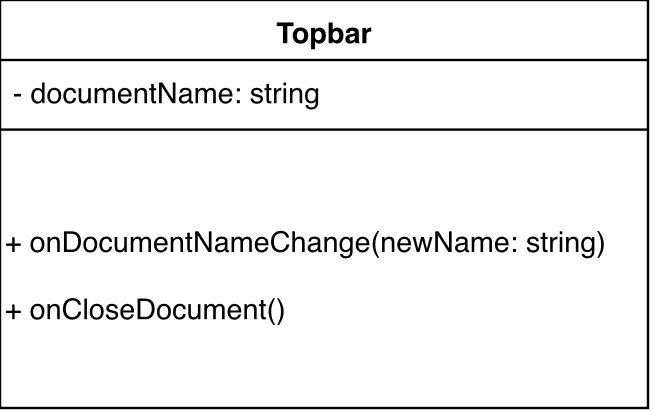
\includegraphics{../UMLimg/TopBar.jpg}
    \caption{UML TopBar}
    \label{fig:uml1.0}
\end{figure}

Il componente Topbar contiene dei pulsanti che consentono di formattare il testo secondo la sintassi \gls{Markdown}.\\

\textbf{Attributi}:
\begin{itemize}
    \item \texttt{documentName:string} - nome del documento
\end{itemize}

\textbf{Metodi}:
\begin{itemize}
    \item \texttt{onDocumentNameChange:(newName:string) => void} - callback per aggiornare il nome del documento
    \item \texttt{onCloseDocument:() => void} - callback per chiudere il documento
\end{itemize}


\subsection{Sidebar}

\begin{figure}[H]
    \centering
    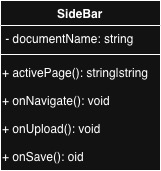
\includegraphics[width=0.8\textwidth]{../UMLimg/SideBar.jpg}
    \caption{UML SideBar}
    \label{fig:uml1.1}
\end{figure}
Il componente Sidebar contiene i pulsanti con le varie funzionalità AI.\\

\textbf{Attributi}:
\begin{itemize}
    \item \texttt{documentName:string} - nome del documento
\end{itemize}

\textbf{Metodi}:
\begin{itemize}
    \item \texttt{activePage:'editor'|'history'} - tipologiia di view visualizzata nel corpo principale della pagina
    \item \texttt{onNavigate:(page:'editor'|'history') => void} - callback per aggiornare la view visualizzata
    \item \texttt{onUpload:() => void} - callback per caricare un documento
    \item \texttt{onSave:() => void} - callback per salvare un documento
    \item \texttt{onPrint:() => void} - callback per stampare un documento
    \item \texttt{onAiAction:() => void} - callback per attivare un'azione AI
\end{itemize}


\subsection{EditorButton}
\begin{figure}[H]
    \centering
    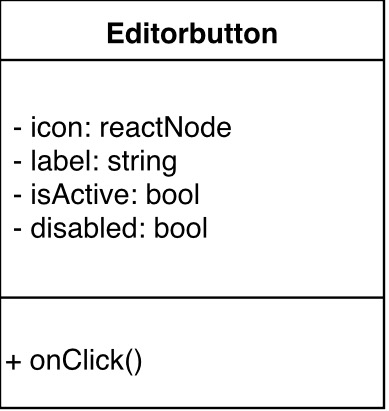
\includegraphics[width=0.8\textwidth]{../UMLimg/EditorButton.jpg}
    \caption{UML EditorButton}
    \label{fig:uml1.2}
\end{figure}
Il componente EditorButton è un bottone che viene utilizzato nella sideBar per i bottoni IA.\\

\textbf{Attributi}:
\begin{itemize}
    \item \texttt{icon:ReactNode} - icona del bottone
    \item \texttt{label:string} - testo del bottone
    \item \texttt{isActive?:boolean} - 
    \item \texttt{disabled?:boolean} - true se il bottone non è cliccabile dall'utente
\end{itemize}

\textbf{Metodi}:
\begin{itemize}
    \item \texttt{onClick:() => void} - callback per gestire il click sul bottone
\end{itemize}


\subsection{SaveDocumentModal}
\begin{figure}[H]
    \centering
    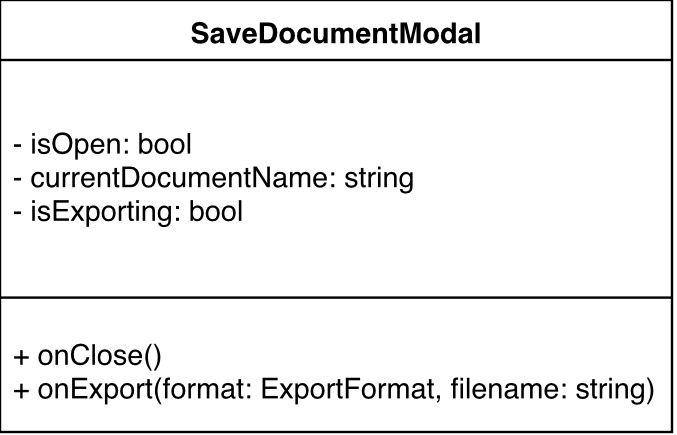
\includegraphics[width=0.8\textwidth]{../UMLimg/SaveDocumentModal.jpg}
    \caption{UML SaveDocumentModal}
    \label{fig:uml1.3}
\end{figure}
Il componente SaveDocumentModal è il componente che rappresenta il modal per il salvataggio del documento.\\

\textbf{Attributi}:
\begin{itemize}
    \item \texttt{isOpen:boolean} - true se il modal è aperto
    \item \texttt{currentDocumentName:string} - nome attuale del documento, da mostrare come placeholder nell'input del nome del documento
    \item \texttt{isExporting?:boolean} - true se il documento è in fase di esportazione, per disabilitare i bottoni
\end{itemize}

\textbf{Metodi}:
\begin{itemize}
    \item \texttt{onClose:() => void} - callback per chiudere il modal
    \item \texttt{onExport:(format:ExportFormat, filename:string) => void} - callback per esportare il documento in un formato specifico
\end{itemize}


\subsection{MarkDownEditor}
\begin{figure}[H]
    \centering
    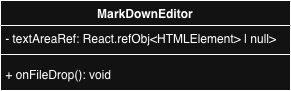
\includegraphics[width=0.8\textwidth]{../UMLimg/MarkDownEditor.jpg}
    \caption{UML MarkDownEditor}
    \label{fig:uml1.4}
\end{figure}
Il componente MarkDownEditor è il componente che rappresenta il corpo principle della pagina e dove viene istanziato \gls{EasyMDE}.\\

\textbf{Attributi}:
\begin{itemize}
    \item \texttt{textAreaRef:\gls{React}.RefObject<HTMLTextAreaElement | null>} - riferimento alla textarea su cui istanziare \gls{EasyMDE}
    
\end{itemize}

\textbf{Metodi}:
\begin{itemize}
    \item \texttt{onFileDrop?:(file:File) => void} - callback per gestire il drop di un file sulla textarea
\end{itemize}


\subsection{HistoryList}
\begin{figure}[H]
    \centering
    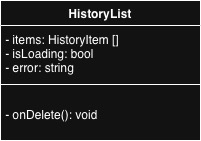
\includegraphics[width=0.8\textwidth]{../UMLimg/HistoryList.jpg}
    \caption{UML HistoryList}
    \label{fig:uml1.5}
\end{figure}
Il componente HistoryList è il componente che rappresenta la lista delle interazioni con l'IA.\\

\textbf{Attributi}:
\begin{itemize}
    \item \texttt{items:HistoryItem[ ]} - lista delle interazioni con l'IA da mostrare nella cronologia
    \item \texttt{isLoading:boolean} - true se la cronologia è in fase di caricamento, per mostrare un indicatore di caricamento
    \item \texttt{error:string | null} - messaggio di errore da mostrare se c'è stato un errore nel caricamento della cronologia
\end{itemize}

\textbf{Metodi}:
\begin{itemize}
    \item \texttt{onDelete:(id:string) => void} - callback per gestire la cancellazione di una interazione dalla cronologia
\end{itemize}


\subsection{HistoryCard}
\begin{figure}[H]
    \centering
    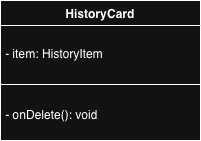
\includegraphics[width=0.8\textwidth]{../UMLimg/HistoryCard.jpg}
    \caption{UML HistoryCard}
    \label{fig:uml1.6}
\end{figure}
Il componente HistoryCard è il componente che rappresenta la scheda di una interazione con l'IA.\\

\textbf{Attributi}:
\begin{itemize}
    \item \texttt{item:HistoryItem}
\end{itemize}

\textbf{Metodi}:
\begin{itemize}
    \item \texttt{onDelete:(id:string) => void} - callback per gestire la cancellazione di una interazione dalla cronologia
\end{itemize}


\subsection{UseEditor}
\begin{figure}[H]
    \centering
    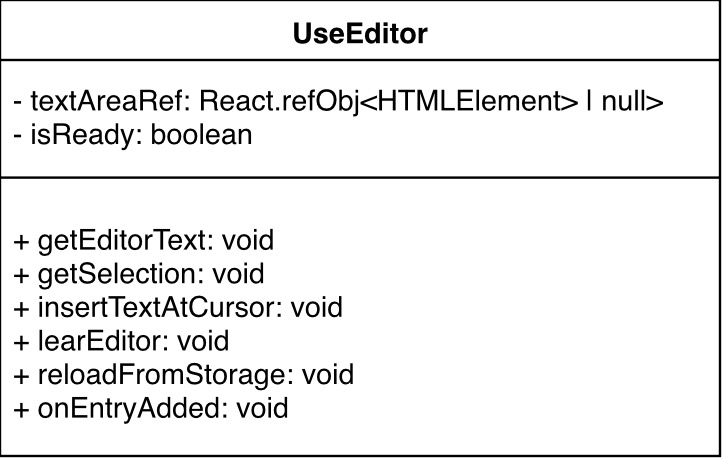
\includegraphics[width=0.8\textwidth]{../UMLimg/UseEditor.jpg}
    \caption{UML UseEditor}
    \label{fig:uml1.7}
\end{figure}
Hook per l'editor\\

\textbf{Attributi}:
\begin{itemize}
    \item \texttt{textArearef: \gls{React}.RefObject<HTMLTextAreaElement | null>} - riferimento alla textarea su cui istanziare \gls{EasyMDE}
    \item \texttt{isReady: boolean} - true quando l'editor è pronto all'utilizzo
\end{itemize}

\textbf{Metodi}:
\begin{itemize}
    \item \texttt{getEditorText: () => string} - restiruisce il testo presente nell'editor
    \item \texttt{getSelection: () => string} - restituisce il testo attualmente selezionato nell'editor
    \item \texttt{insertTextAtCursor: (text: string) => void} - inserisce il testo nella posizione del cursore
    \item \texttt{clearEditor: () => void} - cancella il contenuto dell'editor
    \item \texttt{reloadFromStorage: () => void} - ricarica il contenuto del'editor
    \item \texttt{onEntryAdded?: (entry: unknown) => void} - callback per gestire l'aggiunta di una nuova voce all'editor
\end{itemize}


\subsection{Rappresentazione UML per il frontend}



\newpage

\section{Design Pattern}
\subsection{Strategy pattern}
Il design pattern comportamentale Strategy definisce una famiglia di algoritmi, li incapsula in classi separate e li rende intercambiabili in modo dinamico.

\subsubsection{Problema}
L’architettura iniziale del backend presentava un'eccessiva complessità logica dovuta alla gestione di molteplici modelli LLM e diverse logiche di prompting. La presenza di numerosi blocchi condizionali (if/else o switch) all'interno dell'entry point (\texttt{app.py}) rendeva il codice rigido, difficile da scalare e violava il principio di singola responsabilità (Single Responsibility Principle).


\subsubsection{Applicazione: \gls{prompt} strategies (ai\_strategies.py)}
Questa prima applicazione del pattern gestisce la trasformazione del testo grezzo fornito dall'utente in un input strutturato e ottimizzato per l'IA.

\paragraph{BaseAIStrategy}
Definisce il contratto comune per tutte le strategie di generazione dei \gls{prompt}.
\textbf{Proprietà e Metodi:}
\begin{itemize}
    \item \texttt{temperature}: Definisce il livello di creatività dell'output (es. valori più alti per operazioni creative, più bassi per task analitici).
    \item \texttt{build(text: str)}: Impone a ogni sottoclasse di restituire una tupla contenente due stringhe: il \gls{System prompt} (il ruolo dell'IA) e lo \gls{User prompt} (il task specifico).
\end{itemize}

\paragraph{SimplePromptStrategy}
Utilizzata per le operazioni editoriali standard (riassunto, correzione grammaticale, riscrittura, \gls{distant writing}). Costruisce \gls{prompt} diretti impostando un ruolo e istruzioni ferree per evitare preamboli discorsivi nella risposta dell'IA.
\\ \textbf{Attributi:}
\begin{itemize}
    \item \texttt{role} (str): Definisce l'identità dell'assistente (es. "Sei un correttore di bozze").
    \item \texttt{task} (str): Definisce l'istruzione specifica da eseguire.
\end{itemize}

\paragraph{TranslationStrategy} 
Sottoclasse concreta specializzata nella gestione delle attività di traduzione multilingua. Questa classe ottimizza il \gls{prompt} per garantire che l'LLM operi esclusivamente come traduttore professionale, mantenendo la fedeltà linguistica.\\
\textbf{Attributi:}
\begin{itemize}
    \item language(str): Stringa che definisce la lingua di destinazione (es. "inglese", "cinese mandarino"). Questo attributo viene utilizzato per parametrizzare dinamicamente la richiesta al modello.
\end{itemize}
\textbf{Metodi:}
\begin{itemize}
    \item build(text): Implementa la logica di costruzione del \gls{prompt} impostando un \gls{System \gls{Prompt}} rigido che definisce il ruolo (traduttore professionista) e i vincoli di output (nessuna frase introduttiva). Lo \gls{User \gls{Prompt}} include l'istruzione di traduzione specifica verso la lingua memorizzata nell'attributo language.
\end{itemize}

\paragraph{DeBonoHatStrategy}
Sottoclasse concreta progettata per implementare il metodo dei "Sei Cappelli per Pensare" di Edward de Bono. Questa strategia guida l'LLM verso un'analisi laterale e strutturata, forzando il modello a osservare il testo da una singola prospettiva cognitiva alla volta (emotiva, logica, creativa, ecc.).\\
\textbf{Attributi:}
\begin{itemize}
    \item hat\_name(str): Memorizza il nome o il colore del cappello. Serve a definire l'identità dell'IA.
    \item focus(str): Memorizza l'area di analisi specifica. Serve a guidare il focus del modello durante la generazione.
\end{itemize}
\textbf{Metodi:}
\begin{itemize}
    \item build(self, text): Utilizza le f-string per iniettare i valori di hat\_name e focus all'interno dei \gls{prompt}.
\end{itemize}


\subsubsection{Applicazione: model strategies
(model\_strategies.py)}
Questa seconda applicazione del pattern isola completamente i dettagli tecnici (\gls{Endpoint}, \gls{API} Keys, payload JSON) necessari per comunicare con i diversi provider di Intelligenza Artificiale.

\paragraph{AIModelStrategy} interfaccia comune per tutti i modelli linguistici IA.
\\ \textbf{Metodi:}
\begin{itemize}
    \item generate(self, system\_prompt, user\_prompt): Definisce il contratto per l'invocazione del modello. Ogni classe concreta deve implementare la logica specifica per inviare i \gls{prompt} al fornitore e restituire la risposta come stringa pulita.
\end{itemize}

\paragraph{Implementazioni Concrete (ZucchettiLlamaStrategy e Gemma3Strategy)}
Il sistema prevede due implementazioni concrete che espongono in modo polimorfico i modelli \gls{Llama 3.2} (per operazioni standard e traduzioni) e \gls{Gemma 3} (per il pensiero laterale dei Sei Cappelli).
Entrambe le classi implementano la logica di chiamata \gls{API} (tramite modulo OpenAI compatibile), formattano la richiesta ed estraggono esclusivamente il contenuto testuale della risposta, isolandolo dai metadati di rete.\\
\textbf{Metodi:}
\begin{itemize}
    \item generate(system\_prompt, user\_prompt): Implementa la logica di chiamata \gls{API} tramite il modulo OpenAI, gestisce la struttura della richiesta inviando i due messaggi (System e User) nel formato richiesto dal protocollo ChatCompletion ed estrae e restituisce esclusivamente il contenuto testuale della risposta, isolandolo dai metadati della chiamata (come i token consumati o gli ID di richiesta).
\end{itemize}

\subsubsection{Caching (get\_model)}
La funzione \texttt{get\_model(model\_class)} gestisce un dizionario globale privato (\texttt{\_model\_instances}) per la memorizzazione delle istanze, che funge quindi da cache.
Quando il controller richiede una strategia di modello, la funzione \gls{verifica} se ne esiste già un'istanza nel dizionario: se non esiste, la crea e la salva; alle chiamate successive per la stessa classe, restituisce il riferimento già memorizzato. 
Questa soluzione architetturale ottimizza l'uso delle risorse prevenendo l'apertura di connessioni multiple non necessarie ai client \gls{API}.


\newpage

\subsection{Registry pattern}
Il pattern Registry funge da catalogo centralizzato e configuratore delle operazioni disponibili, disaccoppiando totalmente il Controller (\texttt{app.py}) dalla logica di creazione delle dipendenze.

\subsubsection{Problema}
L’integrazione tra le diverse strategie di prompting e i diversi LLM poneva un problema di accoppiamento rigido e di complessità gestionale. Senza un punto di coordinamento centrale, il Controller avrebbe dovuto:
\begin{itemize}
    \item Conoscere l'esistenza di tutte le classi concrete e importarle direttamente.
    \item Gestire manualmente la logica di accoppiamento tra \gls{prompt} e modelli.
    \item Contenere lunghi blocchi condizionali per istanziare la strategia corretta in base alla stringa ricevuta dal frontend.
\end{itemize}
Questa struttura avrebbe violato il principio di Inversione delle Dipendenze, rendendo l'aggiunta di una nuova operazione un processo rischioso e richiedendo la modifica del codice di routing principale ogni volta che viene introdotta una nuova funzionalità.

\subsubsection{Applicazione: operation\_registry.py}
Il modulo funge da punto di giunzione dell'intera architettura, orchestrando il legame tra le strategie di contenuto (\gls{prompt}) e le strategie di esecuzione (modelli).

\paragraph{OperationConfig} 
La struttura \texttt{OperationConfig} è definita tramite il decoratore \texttt{@dataclass} ed è progettata per garantire un accoppiamento debole tra i componenti. Agisce come un contenitore che incapsula le dipendenze necessarie a ogni singola operazione.\\
\textbf{Attributi:}
\begin{itemize}
    \item \texttt{model\_class} (\texttt{Type[AIModelStrategy]}): è il riferimento al tipo della classe del modello da istanziare, la cui creazione effettiva è delegata al sistema di caching (\texttt{get\_model}) visto in precedenza.
    \item \texttt{\gls{prompt}\_strategy} (\texttt{BaseAIStrategy}): è un'istanza preconfigurata della strategia di \gls{prompt} specifica per quell'operazione.
\end{itemize}

\paragraph{OPERATION\_REGISTRY}
Il nucleo del pattern è implementato come un dizionario globale che associa identificatori testuali univoci (es. \texttt{"summary"}, \texttt{"green\_hat"}) a oggetti \texttt{OperationConfig}. Questa architettura garantisce tre proprietà fondamentali:
\begin{itemize}
    \item \textbf{Adesione al principio Open-Closed}: Per aggiungere una nuova funzionalità è sufficiente registrare una nuova riga nel dizionario di configurazione. Il codice del controller rimane del tutto inalterato, chiuso alle modifiche ma aperto alle estensioni.
    \item \textbf{Routing dinamico dei modelli}: Il registro permette di assegnare il modello LLM più adatto a una specifica operazione. Ad esempio, nel sistema le operazioni editoriali e di traduzione sono instradate nativamente su \gls{Llama 3.2}, mentre le logiche di pensiero laterale dei Sei Cappelli sono delegate a \gls{Gemma 3:4B}.
    \item \textbf{Robustezza e fallback}: In caso di operazione non riconosciuta o assente nel payload della richiesta, il sistema fornisce una configurazione di default in modo trasparente tramite la costante \texttt{DEFAULT\_OPERATION = "summary"}, sfruttando il metodo \texttt{.get()} del dizionario ed evitando crash dell'applicazione.
\end{itemize}



\newpage

\section{Tracciamento dei requisti}
In questa sezione è stato riportato il tracciamento dei requisiti del progetto "Second Brain" con lo scopo di avere una panoramica completa sui requisiti stabiliti nel documento dell'\gls{Analisi dei Requisiti} v.2.0.0 e sul loro conseguimento.

\subsection{Notazione dei requisiti}
Il codice identificativo segue il formato:
\[
R[Importanza]-[Tipo]-[Numero]
\]
Dove le voci assumono i seguenti significati:

\begin{description}
    \item[Importanza] \hfill \\
    Indica il grado di priorità del requisito:
    \begin{itemize}
        \item \textbf{O (Obbligatorio):} Requisito esplicitamente richiesto dall'azienda Zucchetti. La sua mancata implementazione implica il fallimento degli obiettivi primari del progetto.
        \item \textbf{D (Desiderabile):} Requisito non strettamente vincolante ma che il gruppo si impegna ad implementare per migliorare il prodotto.
        \item \textbf{OP (Opzionale):} Requisito di priorità minore, la cui implementazione può essere rimandata.
    \end{itemize}
    
    \item[Tipo] \hfill \\
    Indica la natura del requisito:
    \begin{itemize}
        \item \textbf{F (Funzionale):} Descrive le funzionalità e i servizi che il sistema deve fornire.
        \item \textbf{V (Vincolo):} Descrive limitazioni tecnologiche, normative o implementative imposte esternamente.
        \item \textbf{Q (Qualità):} Descrive le caratteristiche qualitative del sistema (es. performance, sicurezza, manutenibilità).
    \end{itemize}
    
    \item[Numero] \hfill \\
    Un numero intero progressivo univoco per tipologia di requisito.
\end{description}

\subsection{Tracciamento dei requisti funzionali}
\begin{longtable}{|c|p{11cm}|c|}
\hline
\textbf{Codice} & \textbf{Descrizione} & \textbf{Stato}\\
\hline
\endhead
RO-F-1 & Il sistema deve fornire un’area di testo per l’inserimento e la modifica del testo con supporto alla sintassi \gls{Markdown} standard (CommonMark).& Conseguito\\
\hline
RO-F-2 & Il sistema deve informare l’utente con un messaggio in caso di perdita della connessione Internet durante l’utilizzo dell’editor. & ...\\
\hline
RO-F-3 & Il sistema deve informare l’utente con un messaggio se l’editor non risponde ai comandi.& ...\\
\hline
RO-F-4 & L'editor deve compilare la sintassi \gls{Markdown} in tempo reale. & ... \\
\hline
RO-F-5 & Deve essere presente un'area di visualizzazione del documento formattato rispetto alla sintassi \gls{Markdown}. & ... \\
\hline
RO-F-6 & Il sistema deve informare l'utente con un messaggio se il pannello di anteprima non si aggiorna correttamente. & ... \\
\hline
RO-F-7 & Il sistema deve permettere all'utente di selezionare porzioni di testo tramite mouse o tastiera. & ... \\
\hline
RO-F-8 & Il sistema deve permettere all'utente di modificare porzioni di testo selezionate. & ... \\
\hline
RO-F-9 & Il sistema deve permettere all'utente di copiare una parte di testo selezionato. & ... \\
\hline
RO-F-10 & Il sistema deve permettere all'utente di incollare un testo nell'area di testo. & ... \\
\hline
RO-F-11 & Il sistema deve permettere all'utente di tagliare il testo selezionato. & ... \\
\hline
RO-F-12 & Il sistema deve permettere all'utente di annullare l'ultima modifica effettuata. & ... \\
\hline
RO-F-13 & Se non sono presenti operazioni annullabili, il sistema non esegue alcuna azione al comando Undo. & ... \\
\hline
RO-F-14 & Il sistema deve permettere all'utente di ripristinare le modifiche precedentemente annullate. & ... \\
\hline
RO-F-15 & Se non sono presenti operazioni ripristinabili, il sistema non esegue alcuna azione al comando Redo. & ... \\
\hline
RO-F-16 & Nell'editor deve essere presente una barra degli strumenti (\gls{toolbar}) per applicare formattazioni \gls{Markdown} senza scrivere manualmente la sintassi. & ... \\
\hline
RO-F-17 & Il sistema deve permettere l'applicazione del grassetto al testo tramite \gls{toolbar}. & ... \\
\hline
RO-F-18 & Il sistema deve permettere l'applicazione del corsivo al testo tramite \gls{toolbar}. & ... \\
\hline
RO-F-19 & Il sistema deve permettere l'applicazione della sottolineatura al testo tramite \gls{toolbar}. & ... \\
\hline
RO-F-20 & Il sistema deve permettere di creare intestazioni tramite \gls{toolbar}. & ... \\
\hline
RO-F-21 & Il sistema deve permettere l'inserimento di elementi di struttura (tabelle, separatori orizzontali) tramite \gls{toolbar}. & ... \\
\hline
RO-F-22 & Il sistema deve permettere l'inserimento di liste numerate tramite \gls{toolbar}. & ... \\
\hline
RO-F-23 & Il sistema deve permettere l'inserimento di elenchi puntati tramite \gls{toolbar}. & ... \\
\hline
RO-F-24 & Il sistema deve permettere l'inserimento di link e riferimenti tramite \gls{toolbar}. & ... \\
\hline
RO-F-25 & L'utente può applicare più stili contemporaneamente (es. grassetto, corsivo, sottolineatura) alla stessa sezione di testo. & ... \\
\hline
RO-F-26 & L'utente può annullare una formattazione di una porzione di testo selezionato riapplicandola dalla \gls{toolbar}. & ... \\
\hline
RO-F-27 & L'utente può estendere la formattazione a una porzione di testo parzialmente formattato riapplicandola dalla \gls{toolbar}. & ... \\
\hline
RO-F-28 & L'utente può creare sottoliste attivando la creazione di una lista dalla \gls{toolbar} quando il cursore è già all'interno di una lista. & ... \\
\hline
RO-F-29 & L'utente può scegliere una combinazione di formattazioni dalla \gls{toolbar} quando non è presente testo selezionato, per applicarle al testo che scriverà successivamente. & ... \\
\hline
RO-F-30 & Il sistema deve permettere all'utente di selezionare porzioni di testo da inviare all'agente esterno. & ... \\
\hline
RO-F-31 & Il sistema permette di inviare del testo ad un agente esterno. & ... \\
\hline
RO-F-32 & L'utente deve poter accedere alle azioni sul testo tramite agente esterno in ogni momento. & ... \\
\hline
RO-F-33 & Il testo generato viene prima mostrato come proposta, separata visivamente dal testo dell'utente. & ... \\
\hline
RO-F-34 & Il testo in stato di proposta include le opzioni di conferma, annullamento e rigenerazione. & ... \\
\hline
RO-F-35 & Il sistema non permette la modifica del testo generato mentre è in stato di proposta. & ... \\
\hline
RO-F-36 & Il testo generato dall'agente esterno, una volta confermato, viene inserito nella posizione del cursore se presente, altrimenti in fondo al testo. & ... \\
\hline
RO-F-37 & Una proposta che viene confermata viene inserita nel documento nell'editor e la sezione di proposta viene rimossa. & ... \\
\hline
RO-F-38 & Una volta generato e confermato, il testo dell'agente esterno è modificabile tramite le stesse funzionalità dell'editor disponibili per il testo utente. & ... \\
\hline
RO-F-39 & Una proposta annullata comporta la rimozione del testo generato dalla sezione di proposta e la rimozione della sezione stessa. & ... \\
\hline
RO-F-40 & Una proposta che viene rigenerata viene rimandata all'agente esterno con gli stessi parametri e la nuova risposta sovrascrive la proposta corrente. & ... \\
\hline
RO-F-41 & Il sistema deve informare l'utente con un messaggio in caso di errore durante la comunicazione con il servizio LLM. & ... \\
\hline
RO-F-42 & L'utente può annullare un'operazione AI in corso prima del suo completamento. & ... \\
\hline
RO-F-43 & In seguito all'annullamento di un'operazione AI, il documento rimane nello stato precedente alla richiesta. & ... \\
\hline
RO-F-44 & Se la generazione di testo si blocca prematuramente, rimane ciò che è già stato generato, in attesa che l'utente confermi, rigeneri o elimini la proposta. & ... \\
\hline
RO-F-45 & L'agente esterno applica modifiche esclusivamente al testo selezionato dall'utente. Un contesto aggiuntivo può essere fornito solo a scopo interpretativo e non deve essere alterato. & ... \\
\hline
RO-F-46 & L'utente può consultare il registro delle generazioni AI effettuate. & ... \\
\hline
RO-F-47 & Il sistema deve gestire il caso in cui lo storico delle generazioni AI sia vuoto, informando l'utente con un messaggio appropriato. & ... \\
\hline
RO-F-48 & Ogni generazione di testo dell'agente esterno viene inclusa nel registro delle generazioni, incluse quelle annullate dall'utente. & ... \\
\hline
RO-F-49 & Il sistema deve permettere all'utente di visualizzare il testo completo di una generazione dallo storico AI. & ... \\
\hline
RO-F-50 & L'utente deve poter riassumere tutto o una parte selezionata del testo usando un agente esterno. & ... \\
\hline
RO-F-51 & L'utente deve poter usare un agente esterno per riscrivere tutto o una parte selezionata del testo migliorandolo seguendo determinate specifiche come sintassi, stile e chiarezza. & ... \\
\hline
RO-F-52 & L'utente deve poter tradurre il testo usando un agente esterno in: inglese, italiano, tedesco, francese, spagnolo e cinese mandarino. & ... \\
\hline
RO-F-53 & Se l'utente avvia una traduzione senza selezionare la lingua di destinazione, il sistema lo notifica e blocca l'operazione. & ... \\
\hline
RO-F-54 & Il sistema permette di avviare la correzione grammaticale del testo tramite agente esterno. & ... \\
\hline
RO-F-55 & Se non vengono rilevati errori grammaticali, il sistema informa l'utente dell'esito positivo della correzione. & ... \\
\hline
RO-F-56 & Il sistema consente all'utente di avviare l'analisi critica del testo selezionato o dell'intero documento utilizzando il cappello di De Bono scelto. & ... \\
\hline
RO-F-57 & Se il testo è insufficiente per l'analisi critica, il sistema notifica l'utente e interrompe l'operazione. & ... \\
\hline
RO-F-58 & Se l'utente avvia l'analisi critica senza selezionare un cappello di De Bono, il sistema lo notifica e blocca l'operazione. & ... \\
\hline
RO-F-59 & Il sistema permette l'invio di un \gls{prompt} scritto dall'utente per la generazione di testo tramite agente esterno. & ... \\
\hline
RO-F-60 & Il sistema permette la modifica del \gls{prompt} da inviare all'agente esterno prima dell'invio. & ... \\
\hline
RO-F-61 & L'agente esterno può generare testo basandosi su un \gls{prompt} fornitogli dall'utente. & ... \\
\hline
RO-F-62 & Se il \gls{prompt} fornito dall'utente è vuoto o incompleto, il sistema notifica l'utente e impedisce l'invio. & ... \\
\hline
RO-F-63 & L'utente può caricare un file dal proprio dispositivo all'interno dell'editor. & ... \\
\hline
RO-F-64 & Il sistema deve supportare il caricamento di file in formato \gls{Markdown} (\texttt{.md}, \texttt{.\gls{markdown}}) e testo semplice (\texttt{.txt}). & ... \\
\hline
RO-F-65 & Il sistema deve supportare il caricamento tramite dialogo di esplorazione file (file picker). & ... \\
\hline
RO-F-66 & Prima di procedere con il caricamento di un file, il sistema chiede conferma all'utente. & ... \\
\hline
RO-F-67 & Il sistema deve informare l'utente con un messaggio di esito (successo o errore) al termine di ogni tentativo di caricamento file. & ... \\
\hline
RO-F-68 & Il sistema deve validare il formato del file selezionato e impedire il caricamento di formati non supportati. & ... \\
\hline
RO-F-69 & Il sistema deve validare le dimensioni del file selezionato e impedire il caricamento di file che superano la dimensione massima consentita. & ... \\
\hline
RO-F-70 & Il sistema deve impedire il caricamento di file corrotti o illeggibili. & ... \\
\hline
RO-F-71 & Il sistema deve permettere all'utente di rimuovere il file che ha caricato. & ... \\
\hline
RO-F-72 & L'utente può annullare l'operazione di rimozione del file caricato, lasciando l'editor nel suo stato precedente. & ... \\
\hline
RO-F-73 & Il sistema deve essere in grado di convertire il documento da \gls{Markdown} al formato selezionato dall'utente. & ... \\
\hline
RO-F-74 & Il sistema deve permettere di scaricare il file nel dispositivo dell'utente. & ... \\
\hline
RO-F-75 & L'operazione di esportazione o stampa non deve alterare né chiudere il documento originale nell'editor. & ... \\
\hline
RO-F-76 & Il sistema deve informare l'utente con un messaggio di esito al termine di ogni operazione di esportazione. & ... \\
\hline
RO-F-77 & Il sistema deve consentire l'esportazione del documento in formato \gls{Markdown} (\texttt{.md}). & ... \\
\hline
RO-F-78 & Il sistema deve controllare che il range di pagine inserito dall'utente sia valido (non superiore al numero di pagine del documento e non negativo). & ... \\
\hline
RO-F-79 & Il sistema deve permettere di collegare e inviare il documento a un dispositivo di stampa. & ... \\
\hline
RO-F-80 & Il sistema deve informare l'utente con un messaggio in caso di errore durante l'invio del documento alla stampante. & ... \\
\hline
\addlinespace[1em]
\caption{Tracciamento dei \gls{requisiti funzionali}}
\label{tab:tracciamento_requisiti_funzionali}
\end{longtable}

\subsection{Tracciamento dei requisti di qualità}
\begin{longtable}{|c|p{11cm}|c|}
\hline
\textbf{Codice} & \textbf{Descrizione} & \textbf{Stato}\\
\hline
\endhead
RO-Q-1 & Il tempo di risposta dell'interfaccia utente (aggiornamento anteprima, applicazione formattazioni) deve essere inferiore a 500 ms nel 95\% dei casi, misurato su una sessione utente attiva di almeno 30 minuti.  & ... \\
\hline
RO-Q-2 & Il tempo medio di generazione di una risposta da parte del servizio LLM non deve superare i 10 secondi, misurato su un campione di almeno 20 richieste consecutive in condizioni di utilizzo normale.  & ... \\
\hline
RO-Q-3 & Il tasso di errori nelle operazioni principali (salvataggio, apertura file, chiamate AI) non deve superare l'1\%, misurato sul totale delle operazioni eseguite in una sessione utente attiva di almeno 30 minuti. & ... \\
\hline
RO-Q-4 & La percentuale di codice coperta dai test automatici (test coverage) deve essere almeno il 70\%, misurata sull'insieme completo dei moduli rilasciati ad ogni versione. & ... \\
\hline
RO-Q-5 & La complessità ciclomatica (McCabe) di ogni funzione/metodo del codice prodotto non deve superare il valore 8. & ... \\
\hline
RO-Q-6 & La documentazione prodotta deve ottenere un Indice di Gulpease (IG) maggiore o uguale a 40. & ... \\
\hline
RO-Q-7 & Il sistema deve essere sviluppato rispettando le Norme 
di Progetto del gruppo ByteMe. & ... \\
\hline
RO-Q-8 & Il sistema deve essere verificato secondo il Piano di Qualifica prima di ogni rilascio. & ... \\
\hline
RO-Q-9 & Il \gls{manuale utente} deve documentare tutte le funzionalità obbligatorie del sistema e deve ottenere un Indice di Gulpease (IG) maggiore o uguale a 40. & ... \\
\hline
RO-Q-10 & Il manuale di installazione e deployment del sistema deve ottenere un Indice di Gulpease (IG) maggiore o uguale a 40. & ... \\
\hline
\addlinespace[1em]
\caption{Tracciamento dei \gls{requisiti di qualità}}
\label{tab:tracciamento_requisiti_qualità}
\end{longtable}

\subsection{Tracciamento dei requisti di vincolo}
\begin{longtable}{|c|p{11cm}|c|}
\hline
\textbf{Codice} & \textbf{Descrizione} & \textbf{Stato}\\
\hline
\endhead
RO-V-1 & L'applicazione deve essere accessibile tramite browser web. 
I browser supportati sono: Google Chrome ($\geq$ v110), Mozilla Firefox 
($\geq$ v110), Microsoft Edge ($\geq$ v110), Safari ($\geq$ v16). & ... \\
\hline
RO-V-2 & Il sistema deve utilizzare la codifica Unicode (UTF-8) per la rappresentazione interna e lo storage del testo. & ... \\
\hline
RO-V-3 & Il formato di input e di storage del testo deve essere \gls{Markdown}, in conformità allo standard CommonMark. & ... \\
\hline
RO-V-4 & Il sistema deve integrarsi con un servizio LLM tramite \gls{API} REST compatibili con lo standard OpenAI. & ... \\
\hline
\addlinespace[1em]
\caption{Tracciamento dei \gls{requisiti di vincolo}}
\label{tab:tracciamento_requisiti_vincolo}
\end{longtable}

\end{document}